% Options for packages loaded elsewhere
\PassOptionsToPackage{unicode}{hyperref}
\PassOptionsToPackage{hyphens}{url}
\PassOptionsToPackage{dvipsnames,svgnames,x11names}{xcolor}
%
\documentclass[
  11pt,
]{article}

\usepackage{amsmath,amssymb}
\usepackage{setspace}
\usepackage{iftex}
\ifPDFTeX
  \usepackage[T1]{fontenc}
  \usepackage[utf8]{inputenc}
  \usepackage{textcomp} % provide euro and other symbols
\else % if luatex or xetex
  \usepackage{unicode-math}
  \defaultfontfeatures{Scale=MatchLowercase}
  \defaultfontfeatures[\rmfamily]{Ligatures=TeX,Scale=1}
\fi
\usepackage{lmodern}
\ifPDFTeX\else  
    % xetex/luatex font selection
\fi
% Use upquote if available, for straight quotes in verbatim environments
\IfFileExists{upquote.sty}{\usepackage{upquote}}{}
\IfFileExists{microtype.sty}{% use microtype if available
  \usepackage[]{microtype}
  \UseMicrotypeSet[protrusion]{basicmath} % disable protrusion for tt fonts
}{}
\makeatletter
\@ifundefined{KOMAClassName}{% if non-KOMA class
  \IfFileExists{parskip.sty}{%
    \usepackage{parskip}
  }{% else
    \setlength{\parindent}{0pt}
    \setlength{\parskip}{6pt plus 2pt minus 1pt}}
}{% if KOMA class
  \KOMAoptions{parskip=half}}
\makeatother
\usepackage{xcolor}
\usepackage[margin=1in]{geometry}
\setlength{\emergencystretch}{3em} % prevent overfull lines
\setcounter{secnumdepth}{5}
% Make \paragraph and \subparagraph free-standing
\makeatletter
\ifx\paragraph\undefined\else
  \let\oldparagraph\paragraph
  \renewcommand{\paragraph}{
    \@ifstar
      \xxxParagraphStar
      \xxxParagraphNoStar
  }
  \newcommand{\xxxParagraphStar}[1]{\oldparagraph*{#1}\mbox{}}
  \newcommand{\xxxParagraphNoStar}[1]{\oldparagraph{#1}\mbox{}}
\fi
\ifx\subparagraph\undefined\else
  \let\oldsubparagraph\subparagraph
  \renewcommand{\subparagraph}{
    \@ifstar
      \xxxSubParagraphStar
      \xxxSubParagraphNoStar
  }
  \newcommand{\xxxSubParagraphStar}[1]{\oldsubparagraph*{#1}\mbox{}}
  \newcommand{\xxxSubParagraphNoStar}[1]{\oldsubparagraph{#1}\mbox{}}
\fi
\makeatother


\providecommand{\tightlist}{%
  \setlength{\itemsep}{0pt}\setlength{\parskip}{0pt}}\usepackage{longtable,booktabs,array}
\usepackage{calc} % for calculating minipage widths
% Correct order of tables after \paragraph or \subparagraph
\usepackage{etoolbox}
\makeatletter
\patchcmd\longtable{\par}{\if@noskipsec\mbox{}\fi\par}{}{}
\makeatother
% Allow footnotes in longtable head/foot
\IfFileExists{footnotehyper.sty}{\usepackage{footnotehyper}}{\usepackage{footnote}}
\makesavenoteenv{longtable}
\usepackage{graphicx}
\makeatletter
\def\maxwidth{\ifdim\Gin@nat@width>\linewidth\linewidth\else\Gin@nat@width\fi}
\def\maxheight{\ifdim\Gin@nat@height>\textheight\textheight\else\Gin@nat@height\fi}
\makeatother
% Scale images if necessary, so that they will not overflow the page
% margins by default, and it is still possible to overwrite the defaults
% using explicit options in \includegraphics[width, height, ...]{}
\setkeys{Gin}{width=\maxwidth,height=\maxheight,keepaspectratio}
% Set default figure placement to htbp
\makeatletter
\def\fps@figure{htbp}
\makeatother

\usepackage{hyperref}
\usepackage{float}
\hypersetup{
  colorlinks=true,
  linkcolor=blue,
  urlcolor=blue,
  breaklinks=true,
  pdfborder={0 0 0}
}
\makeatletter
\@ifpackageloaded{caption}{}{\usepackage{caption}}
\AtBeginDocument{%
\ifdefined\contentsname
  \renewcommand*\contentsname{Table of contents}
\else
  \newcommand\contentsname{Table of contents}
\fi
\ifdefined\listfigurename
  \renewcommand*\listfigurename{List of Figures}
\else
  \newcommand\listfigurename{List of Figures}
\fi
\ifdefined\listtablename
  \renewcommand*\listtablename{List of Tables}
\else
  \newcommand\listtablename{List of Tables}
\fi
\ifdefined\figurename
  \renewcommand*\figurename{Figure}
\else
  \newcommand\figurename{Figure}
\fi
\ifdefined\tablename
  \renewcommand*\tablename{Table}
\else
  \newcommand\tablename{Table}
\fi
}
\@ifpackageloaded{float}{}{\usepackage{float}}
\floatstyle{ruled}
\@ifundefined{c@chapter}{\newfloat{codelisting}{h}{lop}}{\newfloat{codelisting}{h}{lop}[chapter]}
\floatname{codelisting}{Listing}
\newcommand*\listoflistings{\listof{codelisting}{List of Listings}}
\makeatother
\makeatletter
\makeatother
\makeatletter
\@ifpackageloaded{caption}{}{\usepackage{caption}}
\@ifpackageloaded{subcaption}{}{\usepackage{subcaption}}
\makeatother
\ifLuaTeX
  \usepackage{selnolig}  % disable illegal ligatures
\fi
\usepackage[]{biblatex}
\addbibresource{references.bib}
\usepackage{bookmark}

\IfFileExists{xurl.sty}{\usepackage{xurl}}{} % add URL line breaks if available
\urlstyle{same} % disable monospaced font for URLs
\hypersetup{
  pdftitle={William's Update},
  pdfauthor={William Clinton Co},
  colorlinks=true,
  linkcolor={blue},
  filecolor={Maroon},
  citecolor={blue},
  urlcolor={blue},
  pdfcreator={LaTeX via pandoc}}

\title{William's Update}
\usepackage{etoolbox}
\makeatletter
\providecommand{\subtitle}[1]{% add subtitle to \maketitle
  \apptocmd{\@title}{\par {\large #1 \par}}{}{}
}
\makeatother
\subtitle{Remittances}
\author{William Clinton Co}
\date{September 30, 2025}

\begin{document}
\maketitle
\begin{abstract}
This document is a follow-up to the meeting on September 5th and
addresses the items discussed during that meeting. It provides an update
on current progress of the dataset completion and potential next steps,
while providing an analysis of the current dataset at hand.
\end{abstract}

\renewcommand*\contentsname{Table of contents}
{
\hypersetup{linkcolor=}
\setcounter{tocdepth}{10}
\tableofcontents
}
\setstretch{1}
\section{Introduction}\label{introduction}

\subsection{Data Sources and
Compilation}\label{data-sources-and-compilation}

I received a reply from Mustafizur Rahman, who compiled the South Asian
remittance dataset. I forwarded the reply to you. Overall, they confirm
what we mostly already learned. Next, we will now be talking about
current datasets the we have.

\subsubsection{Potential Data Sources}\label{potential-data-sources}

\begin{itemize}
\tightlist
\item
  \textbf{Bank of Italy}: Rich dataset from 2005-present (quarterly
  frequency)
\item
  \textbf{Italian Provincial Data}: Outgoing remittances by province
  (2011-2024), allowing for \textbf{provincial-level} analysis and
  regressions.

  \begin{itemize}
  \tightlist
  \item
    This is an interesting dataset because it contains outgoing
    remittances at the provincial level, providing additional depth
    compared to our country-level remittance data analysis.
  \item
    Covering the years 2011 to 2024, this dataset reports annual
    outgoing remittance flows, detailing both the Italian province of
    origin and the destination country for each remittance.
  \end{itemize}
\end{itemize}

\subsubsection{Other Data Sources}\label{other-data-sources}

This is the other central bank datasets we have acquired from other
papers and academics.

\begin{itemize}
\tightlist
\item
  Bangladesh Central Bank dataset
\item
  Bank of Italy dataset
\item
  Philippine dataset
\item
  South Asia dataset
\item
  World Bank GDP data (inflation-adjusted, base period 2015)
\end{itemize}

\section{Data Quality Issues and
Corrections}\label{data-quality-issues-and-corrections}

With our current datasets (IMF Kpodar paper and Remitscope), we will
assess their validity. Since the IMF/World Bank produce aggregate
remittance data, we will aggregate our bilateral corridor-level
remittance data and compare the results to these official aggregates.

\subsection{Initial US Outflows
Analysis}\label{initial-us-outflows-analysis}

As discussed in our last meeting, we will now analyze US remittance
outflows.

The initial analysis of US outflows revealed potential data quality
issues:

\begin{figure}[H]

\centering{

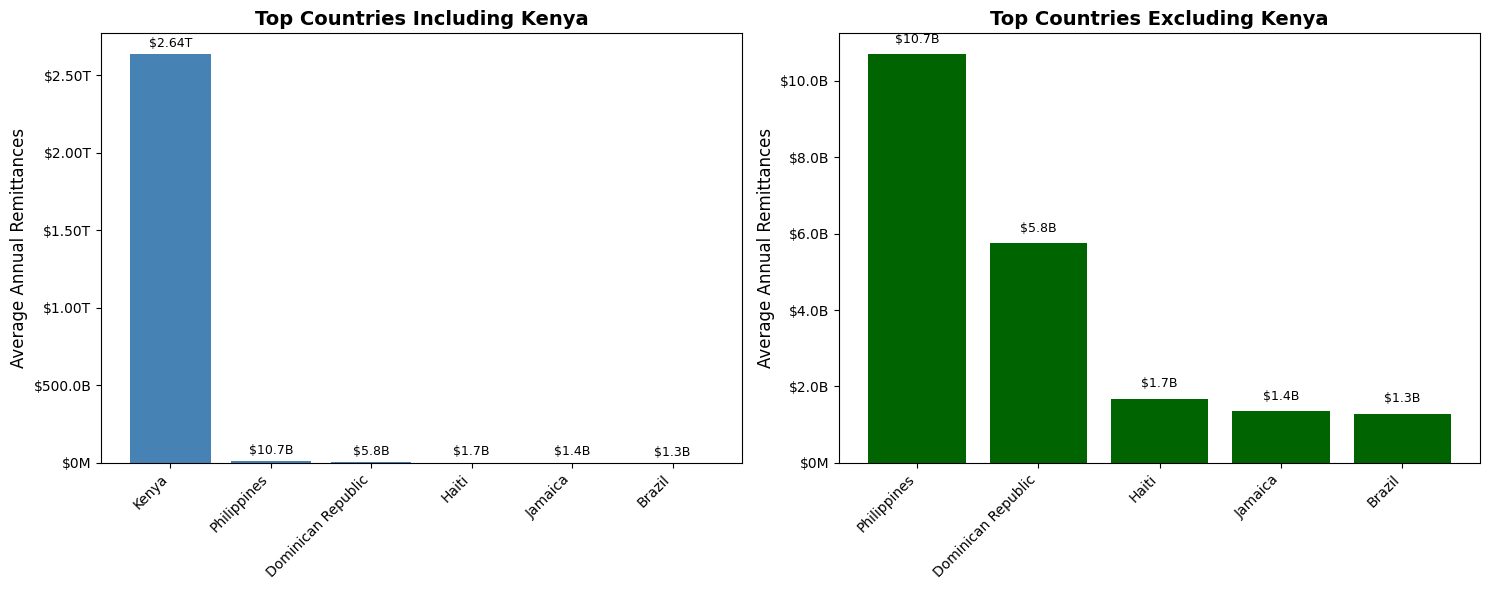
\includegraphics{images/21.png}

}

\caption{\label{fig-us-outflows-initial}Initial US Outflows Analysis}

\end{figure}%

As shown in Figure~\ref{fig-us-outflows-initial}, Kenya appeared
suspiciously high in the remittance flows, prompting further
investigation.

\subsubsection{Kenya Data Correction}\label{kenya-data-correction}

After removing Kenya from the initial analysis, the revised outflows map
showed:

\begin{figure}[H]

\centering{

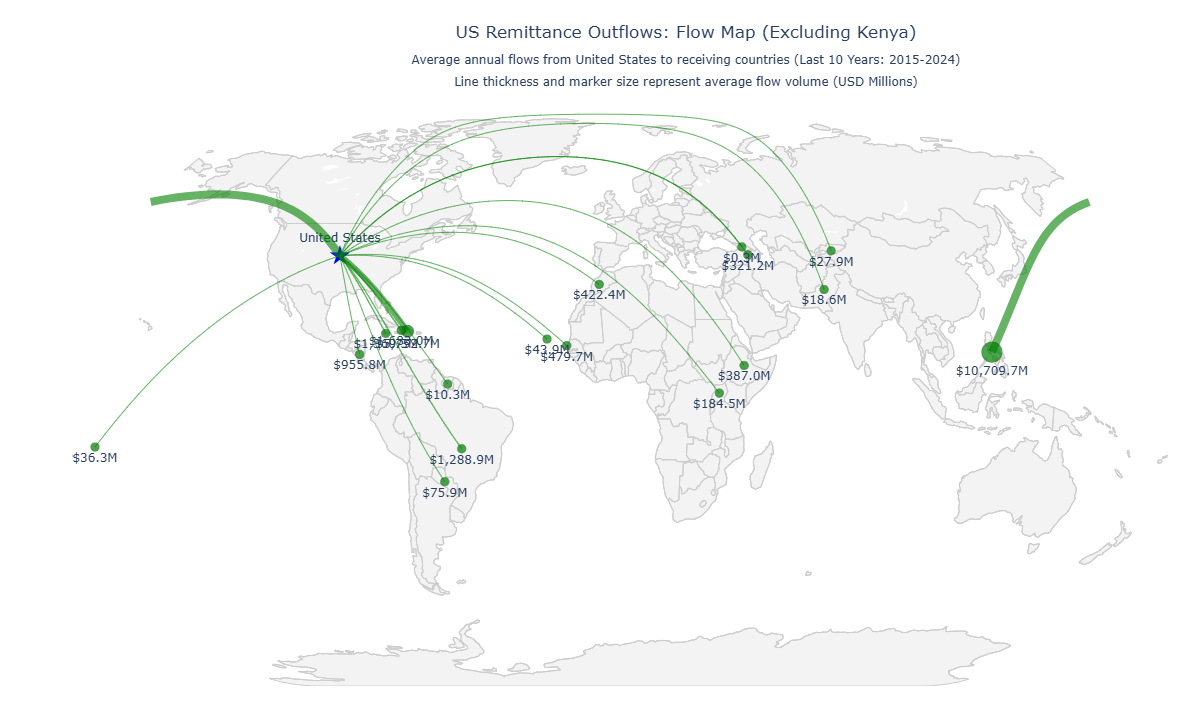
\includegraphics{images/22.png}

}

\caption{\label{fig-us-outflows-no-kenya}US Outflows Analysis (Kenya
Removed)}

\end{figure}%

The detailed interactive map can be accessed at:
\href{https://github.com/WilliamClintC/RER/blob/main/Code/22_flow_map_no_kenya.html}{GitHub
- Interactive Flow Map}

\subsubsection{Data Validation Process}\label{data-validation-process}

Determining the accuracy of individual data points proved challenging.
Cross-referencing with the
\href{https://www.migrationdataportal.org/themes/remittances-overview}{Migration
Data Portal} revealed discrepancies of up to \$1 billion USD in some
cases. These inconsistencies likely stem from a combination of:

\begin{enumerate}
\def\labelenumi{\arabic{enumi}.}
\tightlist
\item
  Known inaccuracies in the World Bank bilateral remittance matrix
\item
  Data collection and reporting errors
\end{enumerate}

\textbf{Kenya Data Verification:}

I verified the Kenya figures against the
\href{https://www.centralbank.go.ke/diaspora-remittances/}{Central Bank
of Kenya's diaspora remittances data}. The comparison revealed:

\begin{itemize}
\tightlist
\item
  Central Bank of Kenya estimate for North America: \textbf{\$2.64
  billion}
\item
  RemitScope dataset figure: \textbf{\$2.64 trillion} (entire order of
  magnitude error)
\end{itemize}

This was not a data scraping error but appeared to be a systematic issue
in the Remitscope data. Evidence suggest this is not a single outlier as
well, which will be seen in later analysis.

\textbf{Data Correction Applied:} I corrected the Kenya data by dividing
by 1,000, resulting in the following US outflow dataset:

\begin{figure}[H]

\centering{

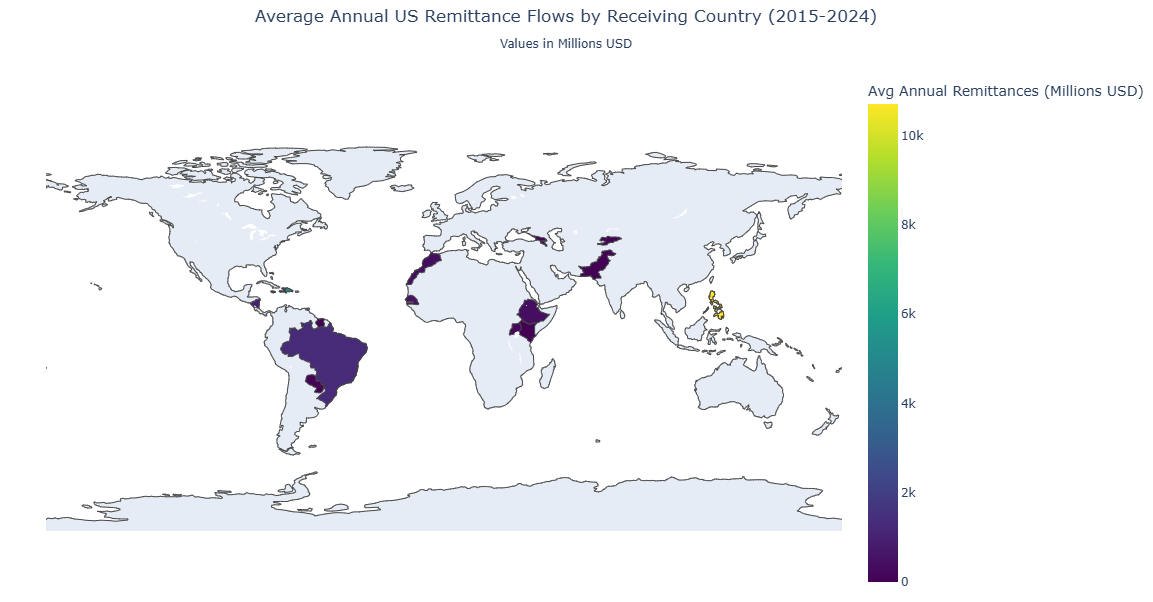
\includegraphics{images/23.png}

}

\caption{\label{fig-us-outflows-corrected}Corrected US Outflows Dataset}

\end{figure}%

\subsubsection{Top Receiving Countries}\label{top-receiving-countries}

The analysis of corrected data reveals the ranking of top
remittance-receiving countries from the United States:

\begin{figure}[H]

\centering{

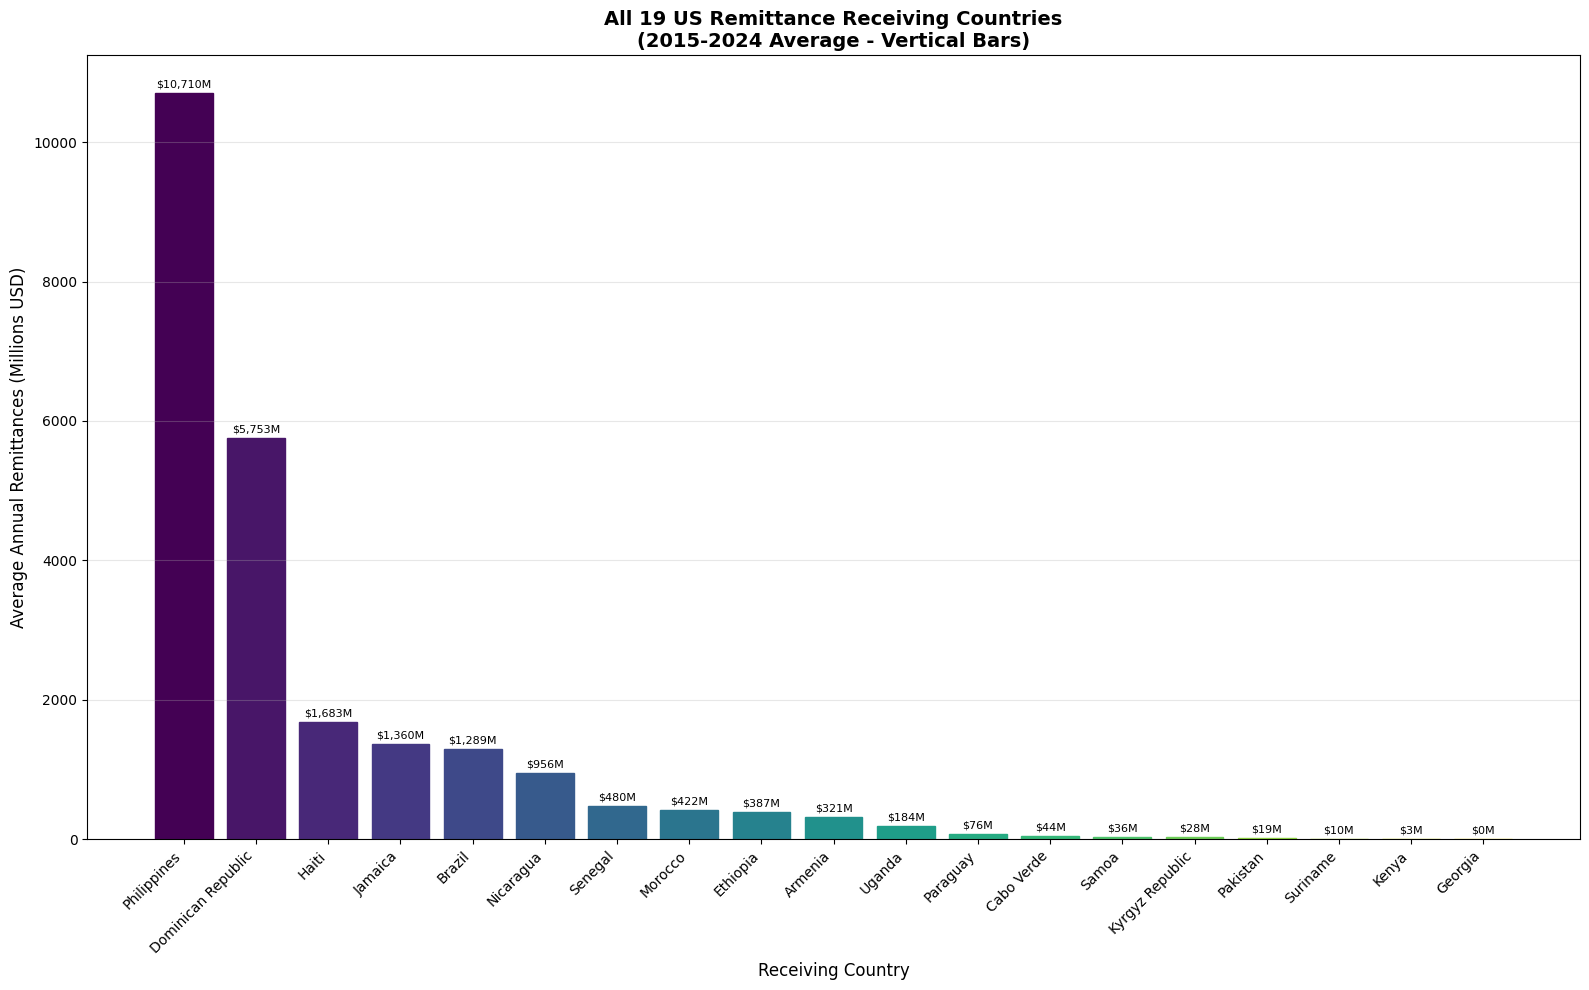
\includegraphics{images/24.png}

}

\caption{\label{fig-top-receiving-countries}Top US Remittance Receiving
Countries}

\end{figure}%

Figure~\ref{fig-top-receiving-countries} illustrates the distribution of
US remittance flows to major receiving countries. The observed results
align with expectations based on established remittance patterns.

To further validate our dataset, we leverage the general accuracy of
macro-level remittance statistics. Accordingly, we aggregate our
bilateral corridor-level data and compare the results to official macro
aggregates (IMF/WorldBank).

Upon aggregating the dataset, it became evident that the discrepancy
associated with Kenya was systematic rather than an isolated , as
illustrated in Figure~\ref{fig-kenya-systematic} .

\begin{figure}[H]

\centering{

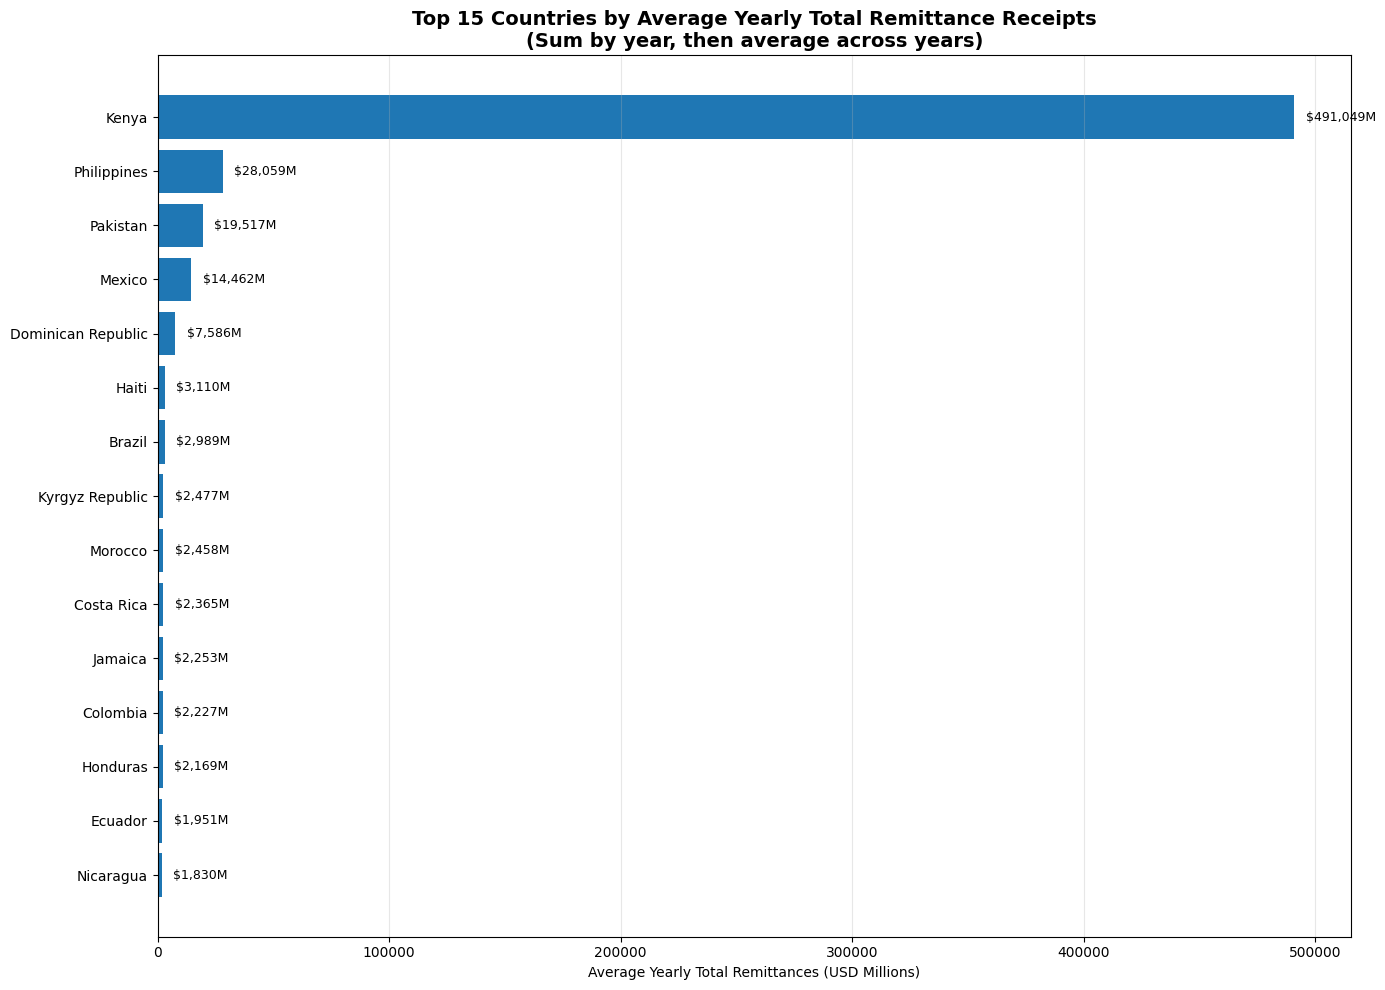
\includegraphics{images/25.png}

}

\caption{\label{fig-kenya-systematic}Kenya Systematic Issue}

\end{figure}%

Specifically, the dataset reported remittance flows to Kenya at
approximately \$491 billion, whereas the World Bank macro remittance
dataset indicates a figure closer to \$4.3 billion USD. This substantial
divergence highlights a persistent issue within the datasets.

To address this, we excluded Kenya from the analysis and employed the
median as a robust measure to mitigate the impact of outliers. The
resulting side-by-side comparison of the datasets is presented in
Figure~\ref{fig-dataset-comparison}.

\begin{figure}[H]

\centering{

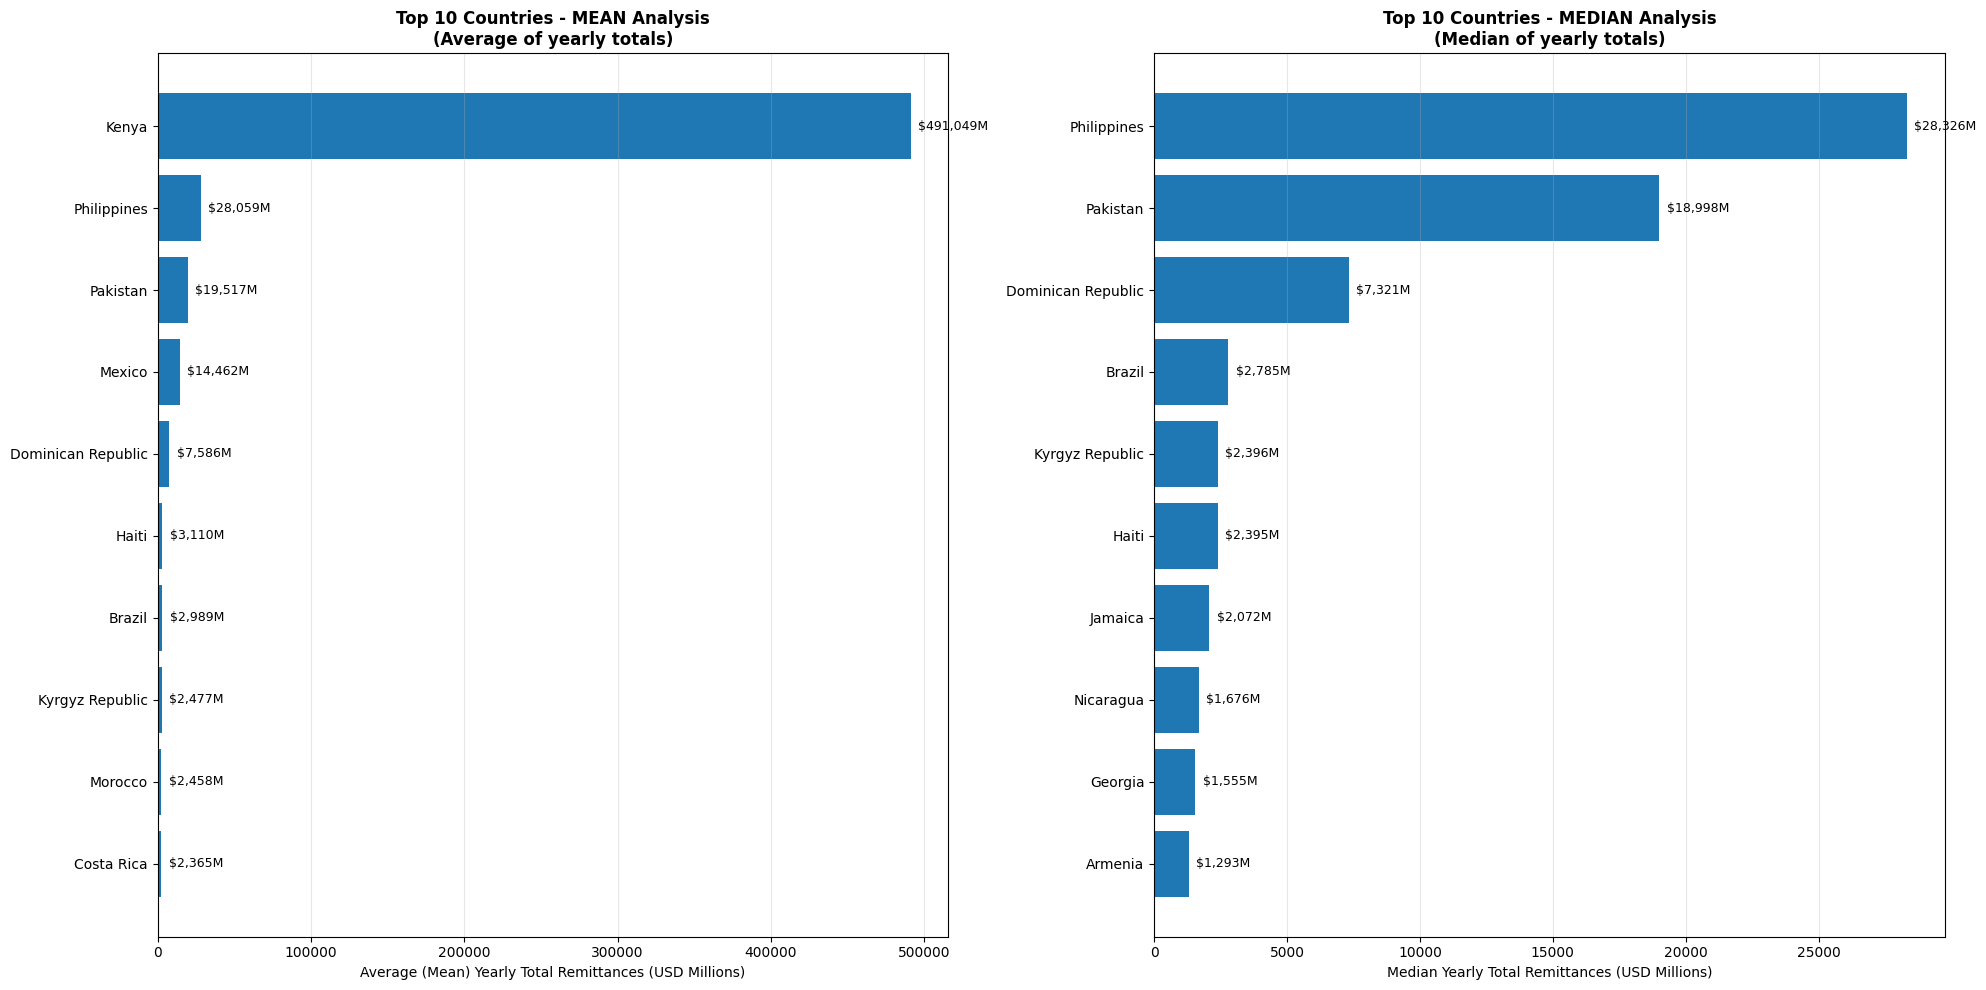
\includegraphics{images/26.png}

}

\caption{\label{fig-dataset-comparison}Dataset Side by Side}

\end{figure}%

Further, Figure~\ref{fig-top30-remittance} displays the top 30
remittance-receiving countries, comparing both the median and mean after
removing Kenya from the sample.

\begin{figure}[H]

\centering{

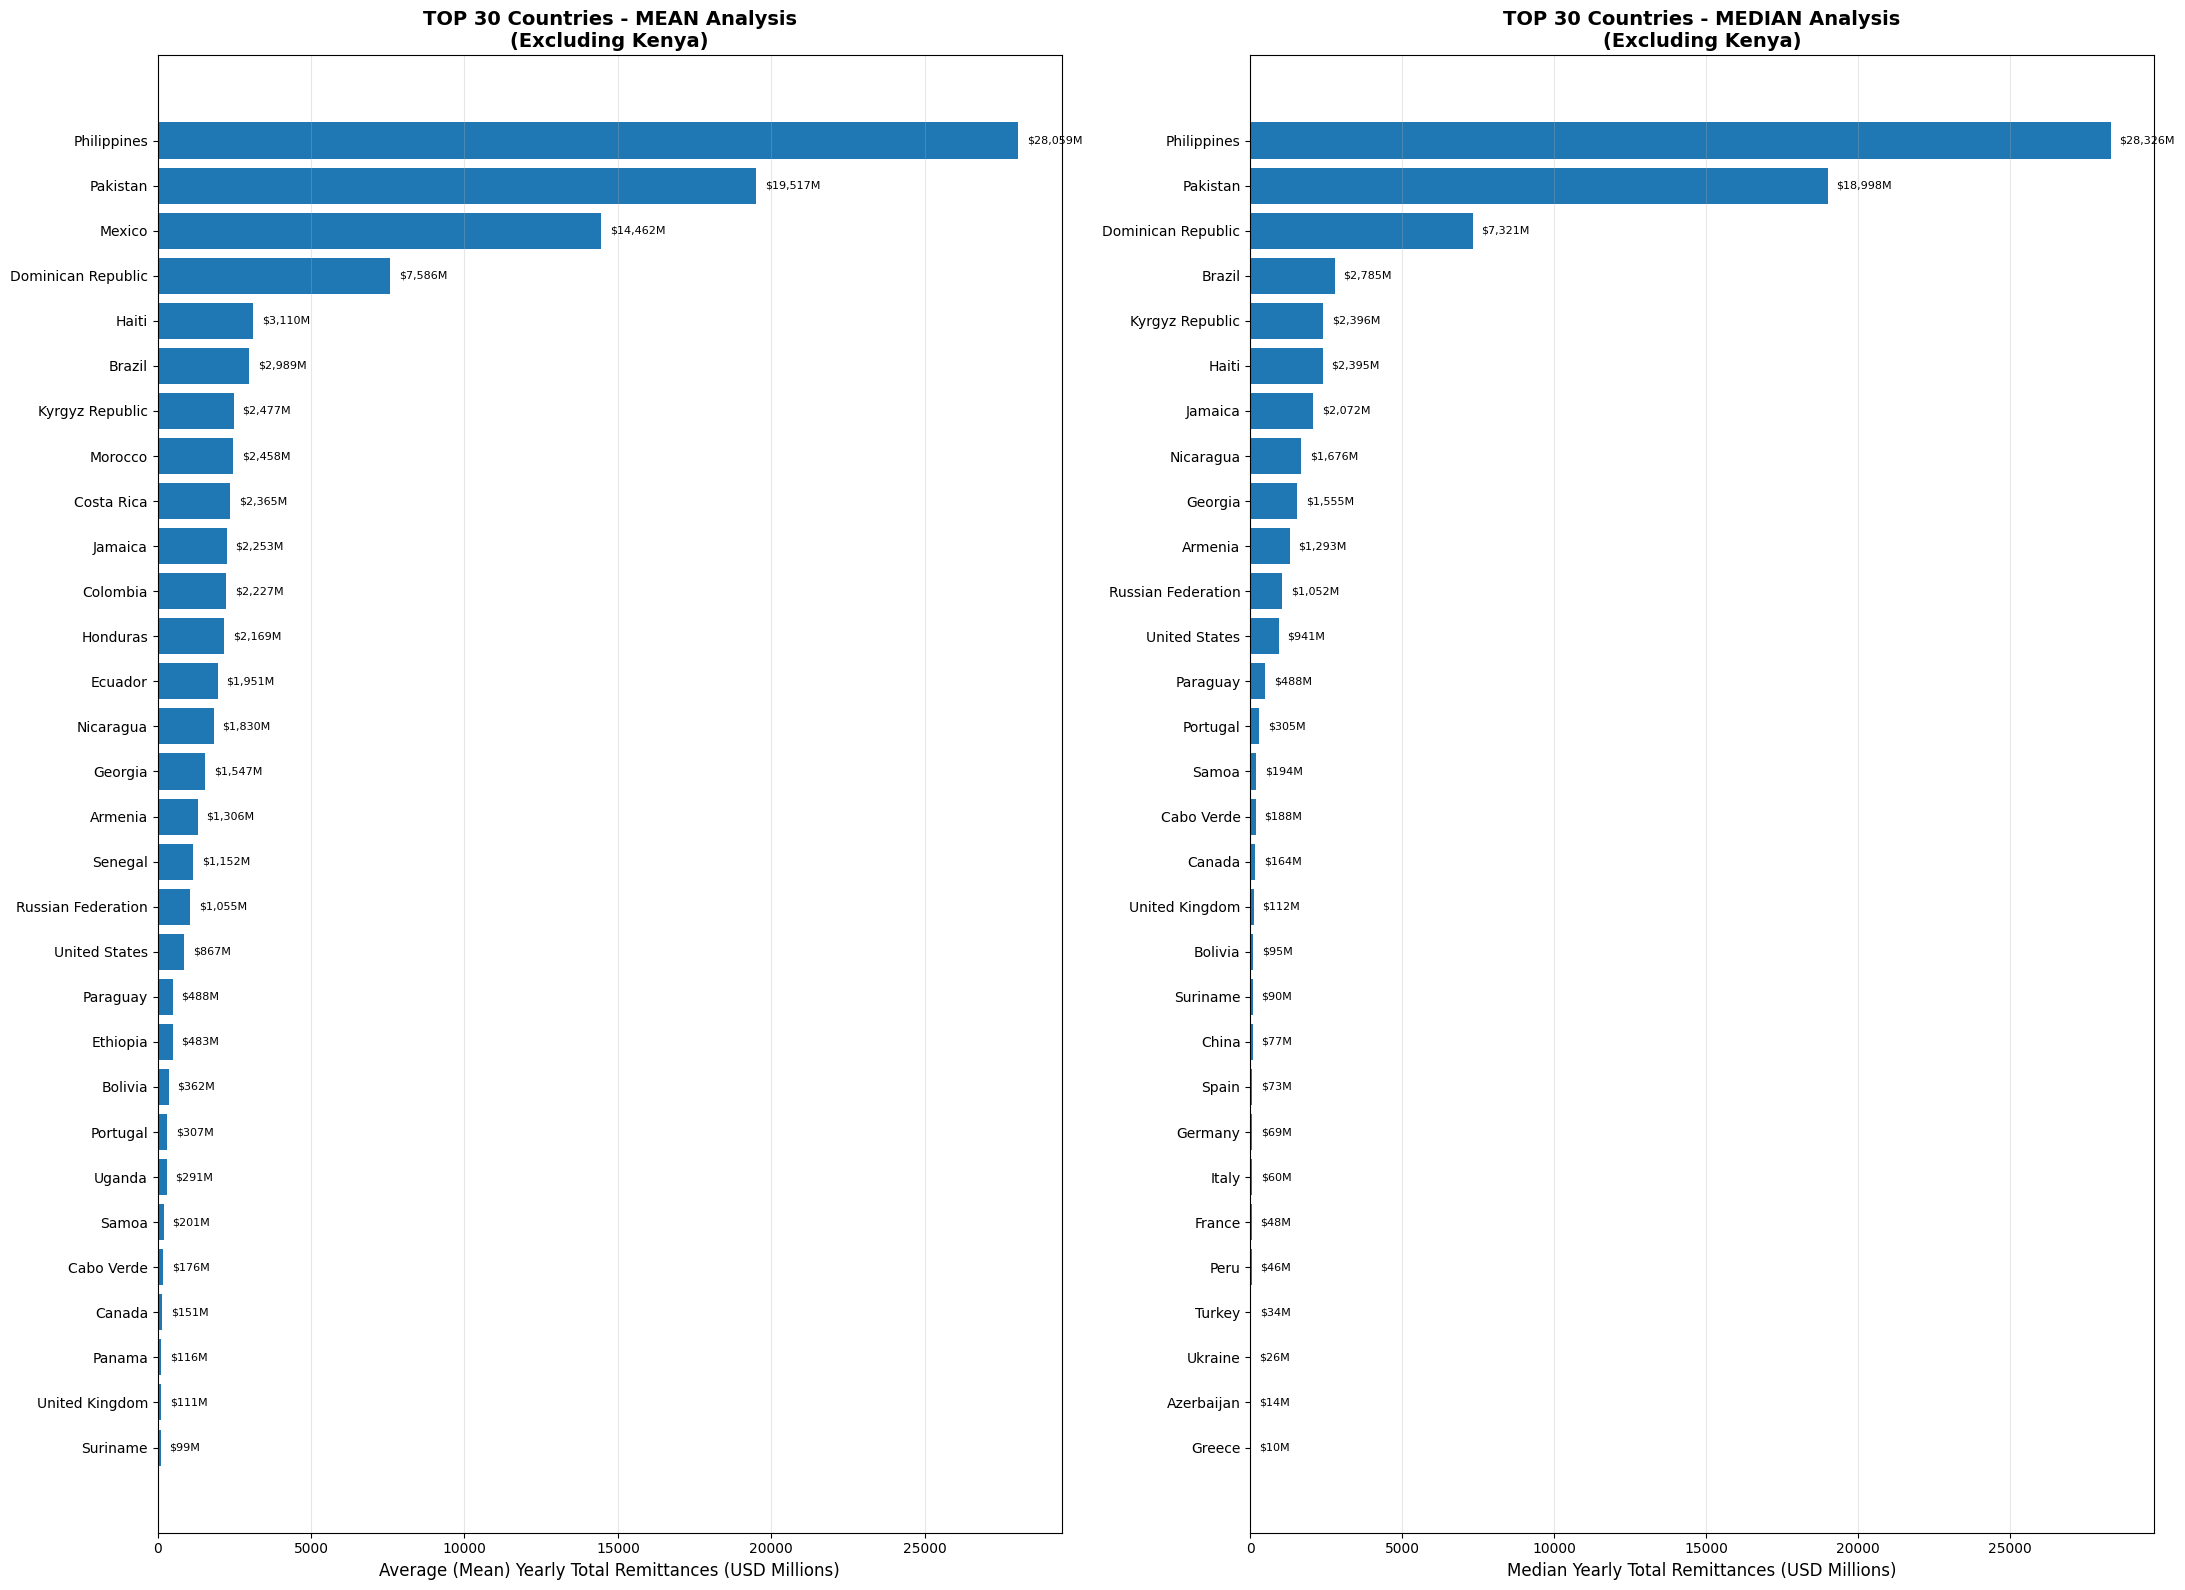
\includegraphics{images/27.png}

}

\caption{\label{fig-top30-remittance}Top 30 Remittance Analysis}

\end{figure}%

\subsection{IMF Macro Remittance vs
Dataset}\label{imf-macro-remittance-vs-dataset}

To assess the consistency of our dataset with established benchmarks, we
compare our remittance estimates to those reported in the IMF macro
remittance dataset. This comparison is conducted across several
dimensions:

\begin{itemize}
\tightlist
\item
  Regional differences are illustrated in
  Figure~\ref{fig-regional-diff}.
\end{itemize}

\begin{figure}[H]

\centering{

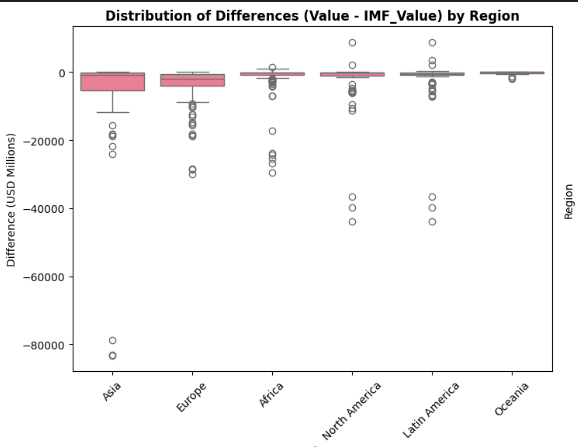
\includegraphics{images/28.png}

}

\caption{\label{fig-regional-diff}Regional Differences}

\end{figure}%

\begin{itemize}
\tightlist
\item
  Temporal differences are presented in Figure~\ref{fig-time-diff}
\end{itemize}

\begin{figure}[H]

\centering{

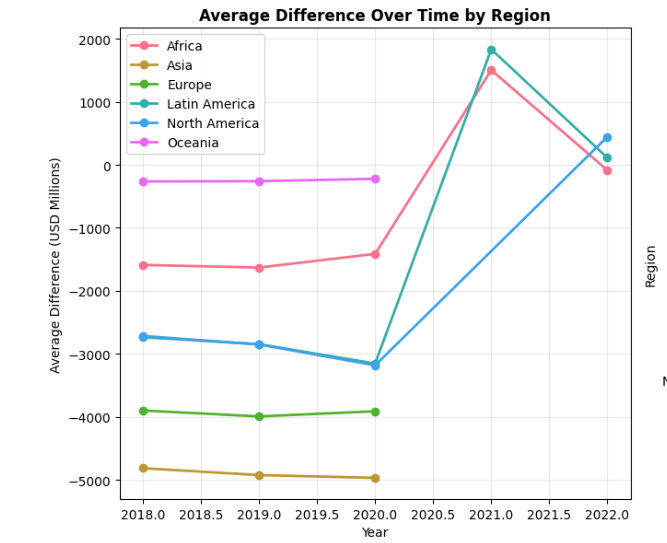
\includegraphics{images/29.png}

}

\caption{\label{fig-time-diff}Time Series Differences}

\end{figure}%

\begin{itemize}
\tightlist
\item
  Combined year and region analysis is shown in
  Figure~\ref{fig-year-region}
\end{itemize}

\begin{figure}[H]

\centering{

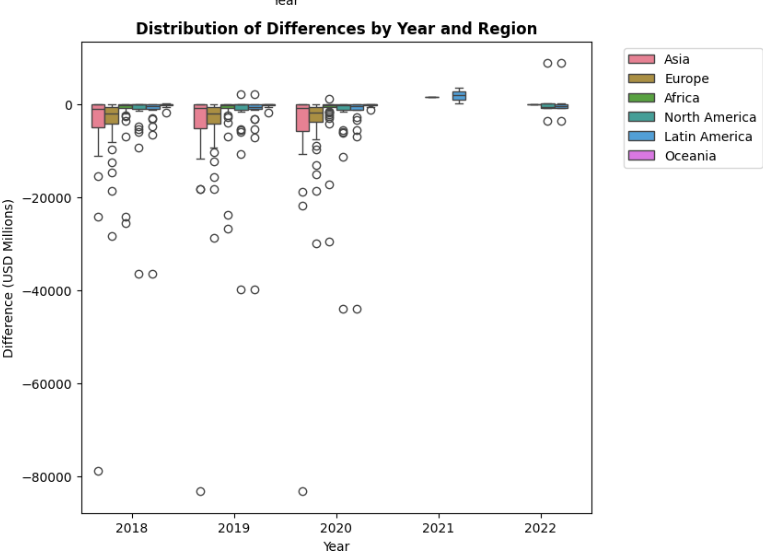
\includegraphics{images/30.png}

}

\caption{\label{fig-year-region}Year and Region Analysis}

\end{figure}%

Next, we sort the data by country to highlight the magnitude of observed
discrepancies. Notably, several countries exhibit substantial
differences, with discrepancies ranging from \$10 billion to \$80
billion USD between our dataset and official macro-level statistics
Figure~\ref{fig-country-discrepancies} :

\begin{figure}[H]

\centering{

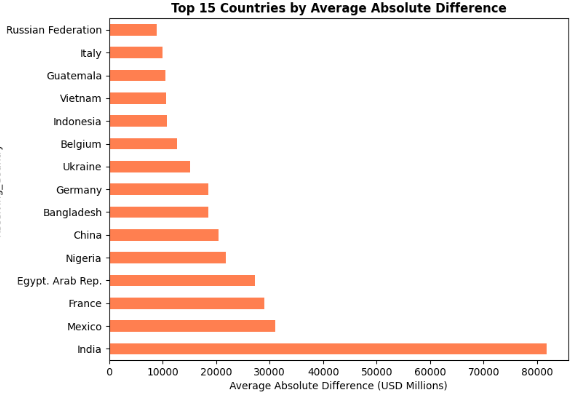
\includegraphics{images/32.png}

}

\caption{\label{fig-country-discrepancies}Country-Level Discrepancies}

\end{figure}%

To further contextualize these discrepancies, we compute the average
difference at the country level. While this approach yields more
moderate values, the discrepancies remain substantial, ranging from
approximately \$1.5 billion to \$3 billion USD. The results are
presented in Figure~\ref{fig-avg-country-discrepancies}.

\begin{figure}[H]

\centering{

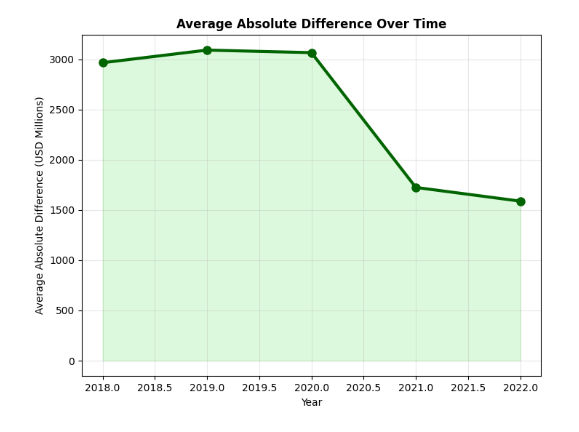
\includegraphics{images/34.png}

}

\caption{\label{fig-avg-country-discrepancies}Average Country
Discrepancies}

\end{figure}%

Given RemitScope's emphasis on Africa and Latin America, we subset our
dataset to focus specifically on these regions. The results of this
regional analysis are presented in Figure~\ref{fig-latam-focus-1} and
Figure~\ref{fig-latam-focus-2}.

\begin{figure}[H]

\centering{

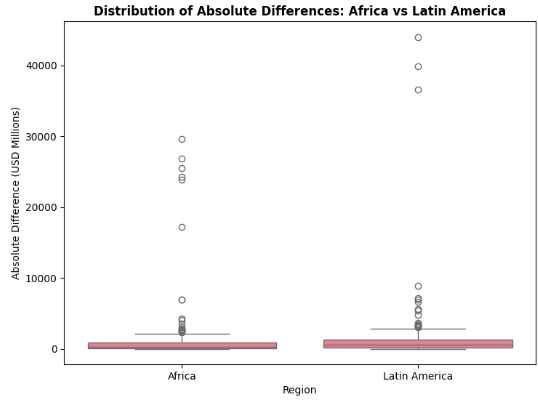
\includegraphics{images/35.png}

}

\caption{\label{fig-latam-focus-1}Latin America Focus 1}

\end{figure}%

\begin{figure}[H]

\centering{

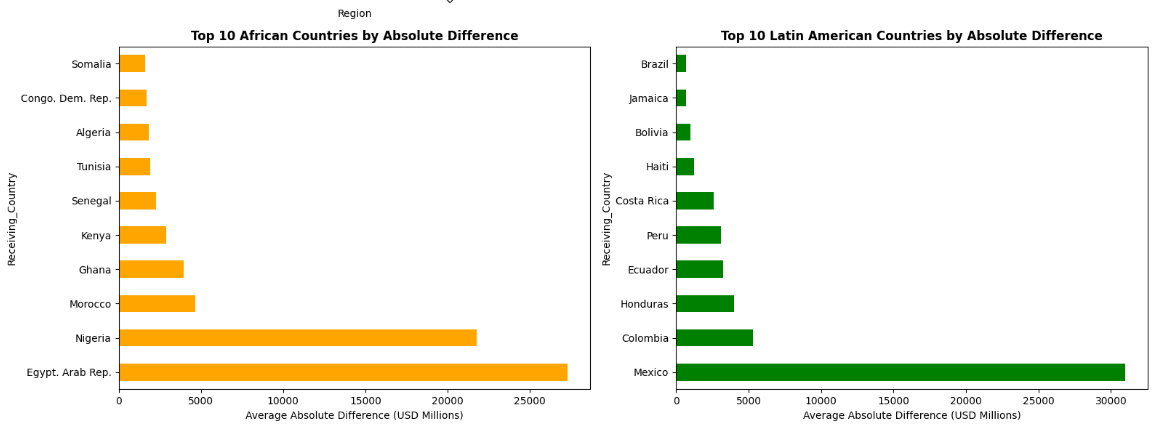
\includegraphics{images/36.png}

}

\caption{\label{fig-latam-focus-2}Latin America Focus 2}

\end{figure}%

To further refine the analysis, we remove prominent outliers such as
Egypt, Nigeria, and Mexico. The impact of this adjustment is shown in
Figure~\ref{fig-outliers-removed-1} and
Figure~\ref{fig-outliers-removed-2}.

\begin{figure}[H]

\centering{

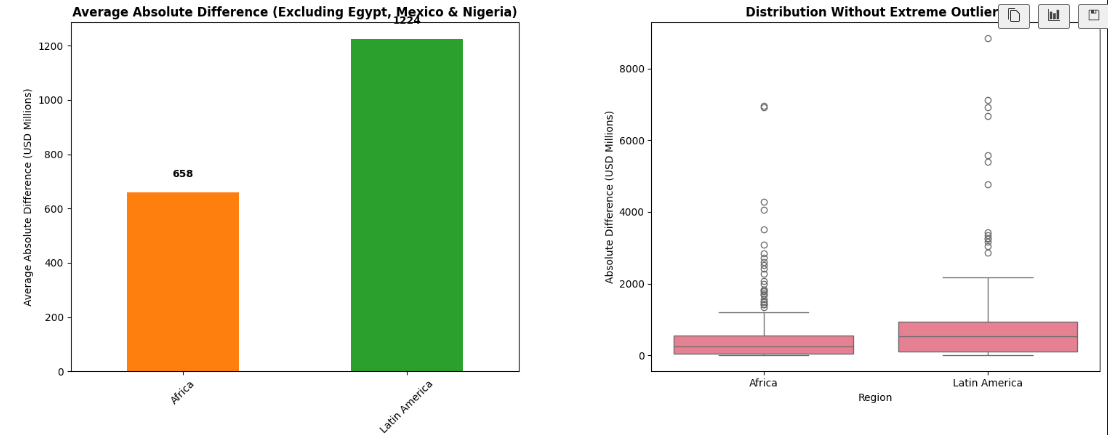
\includegraphics{images/38.png}

}

\caption{\label{fig-outliers-removed-1}Outliers Removed 1}

\end{figure}%

\begin{figure}[H]

\centering{

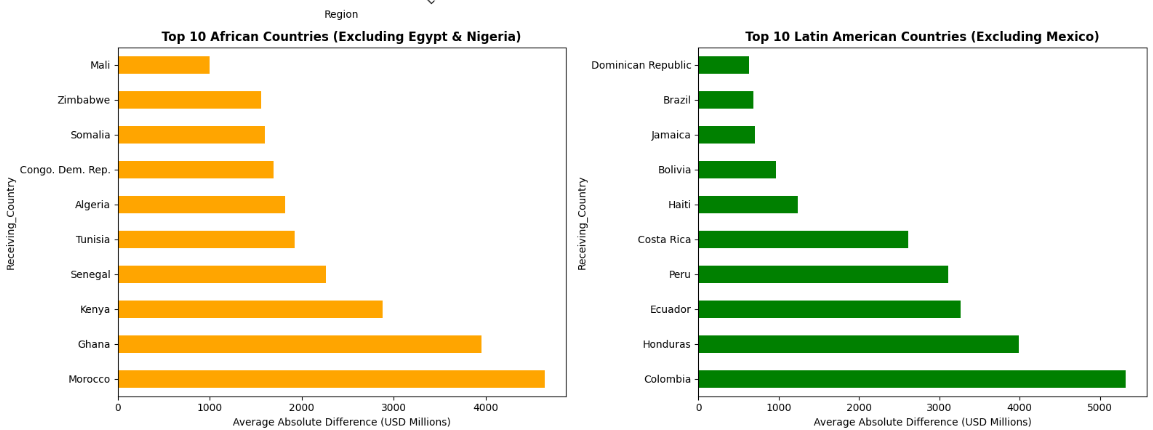
\includegraphics{images/39.png}

}

\caption{\label{fig-outliers-removed-2}Outliers Removed 2}

\end{figure}%

Despite these adjustments, the discrepancies remain substantial, often
exceeding \$1 billion USD. A country-level isolation of the data is
provided in Figure~\ref{fig-country-isolation}.

\begin{figure}[H]

\centering{

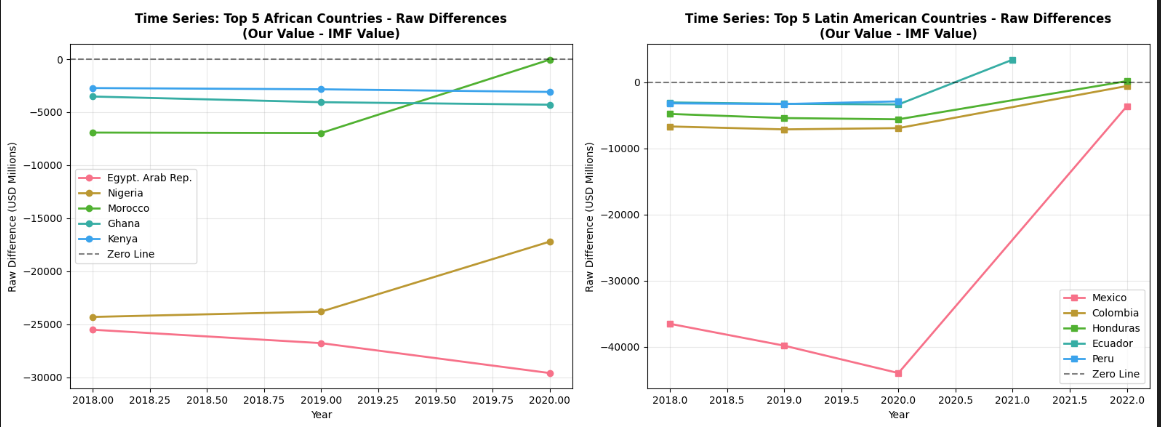
\includegraphics{images/40.png}

}

\caption{\label{fig-country-isolation}Country Isolation}

\end{figure}%

These errors can be partially attributed to several factors: 1.
Discrepancies in macro-level data sources may arise due to differences
in reporting standards and aggregation methods. 2. Data encoding errors
within RemitScope can introduce inconsistencies (as shown with Kenya).
3. Central bank datasets often prioritize major remittance corridors,
frequently excluding countries with minimal remittance flows. As a
result, published data may only reflect the top 20 remitting countries
or similar subsets.

In summary, while the dataset exhibits notable discrepancies, these
issues can be managed through careful methodological adjustments.

\subsection{Empirical Analysis: Drivers of
Remittances}\label{empirical-analysis-drivers-of-remittances}

With the corrected dataset, I proceed to analyze the determinants of
remittance flows through regression analysis.

\subsection{Econometric
Specifications}\label{econometric-specifications}

The GDP mapping process was challenging due to unstructured data, but I
successfully completed it. \#\#\# Linear Model (Levels)

For comparison purposes, I estimate a linear specification in levels:

\begin{equation}\phantomsection\label{eq-linear}{
\text{Remit}_{ij,t} = \alpha_0 + \alpha_1 \text{GDP}_{\text{sender},i,t} + \alpha_2 \text{GDP}_{\text{receiver},j,t} + u_{ij,t}
}\end{equation}

Where:

\begin{itemize}
\tightlist
\item
  Dependent variable: \textbf{Remittances (level)} in millions USD
\item
  \(\alpha_1\) and \(\alpha_2\) measure the \textbf{marginal change} in
  remittances for a one-unit change in GDP (e.g., \$1 billion)
\item
  \(u_{ij,t}\) is the error term
\end{itemize}

\subsubsection{Log-Log (Gravity) Model}\label{log-log-gravity-model}

Following the gravity model literature, I estimate a log-linear
specification:

\begin{equation}\phantomsection\label{eq-gravity}{
\ln(\text{Remit}_{ij,t}) = \beta_0 + \beta_1 \ln(\text{GDP}_{\text{sender},i,t}) + \beta_2 \ln(\text{GDP}_{\text{receiver},j,t}) + \varepsilon_{ij,t}
}\end{equation}

Where:

\begin{itemize}
\tightlist
\item
  Dependent variable: \(\ln(\text{Remittances})\)
\item
  Key independent variables: \(\ln(\text{GDP}_{\text{sender}})\),
  \(\ln(\text{GDP}_{\text{receiver}})\)
\item
  \(\varepsilon_{ij,t}\) is the error term
\end{itemize}

\textbf{Interpretation:}

\begin{itemize}
\tightlist
\item
  \(\beta_1\) = elasticity of remittances with respect to \textbf{sender
  GDP}
\item
  \(\beta_2\) = elasticity of remittances with respect to
  \textbf{receiver GDP}
\end{itemize}

The gravity model specification allows for percentage interpretations: a
1\% increase in sender GDP leads to a \(\beta_1\)\% change in
remittances, holding receiver GDP constant.

\subsection{Unlagged Model}\label{unlagged-model}

A baseline specification can be written as:

\[
Remittances_{i,t} = \alpha 
+ \beta_1 \, GDP^{sending}_{i,t} 
+ \beta_2 \, GDP^{receiving}_{i,t} 
+ \epsilon_{i,t}
\]

where:

\begin{itemize}
\tightlist
\item
  \(Remittances_{i,t}\) = remittance inflows from country \(i\) at time
  \(t\)\\
\item
  \(GDP^{sending}_{i,t}\) = GDP of the migrant-hosting (sending)
  country\\
\item
  \(GDP^{receiving}_{i,t}\) = GDP of the migrant-origin (receiving)
  country\\
\item
  \(\epsilon_{i,t}\) = error term
\end{itemize}

\begin{center}\rule{0.5\linewidth}{0.5pt}\end{center}

\subsection{Lagged Model}\label{lagged-model}

To reduce concerns about reverse causality (i.e., remittances also
influencing GDP), we can use lagged GDP values:

\[
Remittances_{i,t} = \alpha 
+ \beta_1 \, GDP^{sending}_{i,t-1} 
+ \beta_2 \, GDP^{receiving}_{i,t-1} 
+ \epsilon_{i,t}
\]

In this model, current remittances are explained by \emph{past} GDP
levels in both the sending and receiving countries. This assumes that
today's remittances cannot affect yesterday's GDP.

\begin{center}\rule{0.5\linewidth}{0.5pt}\end{center}

\subsection{Extensions}\label{extensions}

Additional control variables may be added to improve robustness, for
example:

\begin{itemize}
\tightlist
\item
  Exchange rate: \(ExRate_{i,t}\)\\
\item
  Migrant stock: \(MigrantStock_{i,t}\)\\
\item
  Unemployment in sending country: \(Unemp^{sending}_{i,t}\)
\end{itemize}

A more general model could look like:

\[
Remittances_{i,t} = \alpha 
+ \beta_1 \, GDP^{sending}_{i,t-1} 
+ \beta_2 \, GDP^{receiving}_{i,t-1} 
+ \beta_3 \, ExRate_{i,t} 
+ \beta_4 \, MigrantStock_{i,t} 
+ \epsilon_{i,t}
\]

\begin{center}\rule{0.5\linewidth}{0.5pt}\end{center}

\subsection{Interpretation}\label{interpretation}

\begin{itemize}
\tightlist
\item
  \(\beta_1 > 0\): Higher GDP in the sending country increases
  remittance flows.\\
\item
  \(\beta_2 < 0\): Higher GDP in the receiving country reduces the need
  for remittances.\\
\item
  \(\beta_3\) and \(\beta_4\): Context-dependent but expected to be
  positive in most cases.
\end{itemize}


\printbibliography


\end{document}
